\documentclass[11pt]{article}
\usepackage[a4paper,margin=1.6cm]{geometry}
\usepackage{fontspec}
\usepackage{xeCJK}
\setCJKmainfont{WenQuanYi Micro Hei}[AutoFakeBold=2.5]
\setmainfont{TeX Gyre Termes}
\usepackage{booktabs}
\usepackage{longtable}
\usepackage{array}
\usepackage{caption}
\usepackage{graphicx}
\usepackage{hyperref}
\usepackage{setspace}
\setstretch{1.12}
\hypersetup{colorlinks=true,linkcolor=black,urlcolor=blue}
\begin{document}
{\centering\Large SelectiveMine Geometry Relay 的重新训练消融\par}
\vspace{0.6em}
本文报告 Geometry Relay 在同一训练预算下的重新训练对照、机制对照、场景分组、参数量、显存、单张耗时和可视化。主指标是测试集 16 类像素准确率、平均像素准确率和平均交并比。16 类把标签 0 计入，标签 255 忽略。15 类同时忽略标签 0 和 255，只作对照。百分比由 JSON 中的原始分数换算，均值旁边的数是三种子的样本标准差。先前对 selective\_pa3 第 12 轮冻结权重做推理消融时，去掉 Relay 后测试集 16 类像素准确率、平均像素准确率和平均交并比的差值都是 0.00、0.00 和 0.00 个百分点。那个结果只说明当前权重和当前推理代码没有使用 Relay 改变输出，不能说明重新训练之后 Relay 没有作用，也不能说明它有作用。

\section*{1  协议}
数据根目录是 /root/autodl-tmp/MUSeg/flat。划分文件是 FTransUNet 的 train.txt、val.txt 和 test.txt，图像数分别是 1595、788 和 788，三个名单交集为 0。所有变体从 selective\_ftrans 的同一份检查点出发，训练 12 轮，输入 768×896，批大小 4，初始学习率 6e-6，余弦调度下限为 0.05 倍。损失与 selective\_pa3 相同：选择性损失的外观、融合、几何和路由器权重是 0.5、0.5、0.2 和 0.05，另加权重 0.25 的 Lovász，以及权重 0.12 的像素负对数似然。背景类权重乘数是 1.15。稀有类裁剪概率是 0.40。随机种子是 2026、2027 和 2028。cudnn.benchmark 与原先的微调脚本一样打开，所以同一种子不保证逐位复现，三种子用来观察方向是否稳定。发行推理包把融合方式建成 logits，Relay 的输出卷积在 selective\_ftrans 第 7 轮里仍是全 0，所以把它接进前向之前不会改变预测。本次完整模型把融合方式设为 relay，让这块模块真正接受梯度。为了在批大小仍是 4 时放进 32 GB 显存，反向时重算 RGB 编码器的激活。损失、优化器和选择规则不变。十八次训练在 RTX 5090 上于 2026-11-02 12:07 全部结束。主流程当时还没有进入测试评估，脚本在循环结束后读到了被改写的内容，报出 cho: command not found 和 syntax error near unexpected token done，然后退出。12:51 监测发现结果包不存在，发出失败邮件并关机。恢复时没有重新训练，沿用这十八份只按验证集选定的权重。测试集在恢复之后才第一次计算。恢复评估使用 RTX 4090，推理不反传，批大小仍是 4。

模型选择只看验证集。规则是 select-pa：在 16 类平均交并比不低于 60.80\% 且平均像素准确率不低于 72.00\% 的轮次中，保留 16 类像素准确率最高的一轮。若没有任何一轮同时达到两道地板，则改用验证集 16 类平均交并比最高的一轮，并在选择表中标明。这个后备规则在测试之前写定，仍然不看测试集。测试集只在全部权重选定之后评估一次。

判读规则在查看测试分数之前写定。某种子差定义为该变体减去完整模型。若 mIoU 差的均值绝对值小于 0.20 个百分点，且样本标准差小于 0.50 个百分点，记为差异很小。若三种子同号，且均值绝对值大于样本标准差，记为方向稳定。其余记为不稳定。只有去掉 Relay 的 mIoU 差方向稳定时，才根据场景表讨论 Relay 在哪些条件下更高。稳定为负表示去掉 Relay 后更低，也就是完整模型更高。

场景阈值来自验证集，写在 0.769433 的深度有效比例中位数、亮度 20 分位 0.096190、亮度 50 分位 0.182265、以及有效深度 75 分位 2616 毫米。验证集落入高、低有效深度的图像数是 394 和 394；低照度和正常照度是 158 和 394。低照度与正常照度之间的图像不进入这两个组。远距离、小目标、深度空洞邻域和语义边界是像素组，阈值分别是 2616 毫米、连通域面积 2048、膨胀半径 8 和 3。几何结构类是管路、轨道区域、支护设备、门、金属构件和锚固设备。外观纹理类是人员、线缆、指示装置、电气设备、电子设备、采掘设备、工具材料、救援设备和容器。这两组按类别定义事先划分，不按测试分数挑选。

{\footnotesize\setlength{\tabcolsep}{3pt}
\begin{longtable}{lc}
\caption*{表 1  一次只改一个因素。}\\
\toprule
变体 & 相对完整模型的改动\\
\midrule
\endfirsthead
\toprule
变体 & 相对完整模型的改动\\
\midrule
\endhead
完整模型 & 保留 Geometry Relay，几何输入为 HHA。\\
去掉 Relay 并重训 & 前向不调用 Relay，Relay 参数不加入优化器。深度门控、HHA 几何头和路由器保留。\\
有效性掩码为常数 & 只把 Relay 内部的深度有效掩码换成全 1。覆盖度变为 1 后，推断支路乘上的 (1-覆盖度) 为 0，空洞不再写入传递特征。网络其余部分仍使用真实掩码。\\
关闭邻域传递 & Relay 的卷积和参数量保持不变，偏移只保留中心点。查询、键、值和后续卷积仍执行，但邻域像素不再进入传递结果。\\
原始深度代替 HHA & 几何输入改为对数深度复制成三通道，按与 HHA 相同的均值和方差缩放，再拼上有效掩码，凑成茎网络要求的四通道。不使用高度和法向角。\\
去掉几何输入 & HHA 位置换成全 0。Relay、几何编码器和几何头仍在，只是几何输入为空。\\
\bottomrule
\end{longtable}}
\section*{2  验证集选择}
下表是每个种子实际保存的轮次。地板未达到时，使用事先规定的验证集平均交并比后备，不改用测试集。

{\footnotesize\setlength{\tabcolsep}{3pt}
\begin{longtable}{lccccccc}
\caption*{表 2  验证集选择。PA、MPA、mIoU 是该轮验证集的 16 类分数，单位是百分比。最后一列是重评与保存分数的 mIoU 绝对差。}\\
\toprule
变体 & 种子 & 轮次 & 达到地板 & PA & MPA & mIoU & 重评差\\
\midrule
\endfirsthead
\toprule
变体 & 种子 & 轮次 & 达到地板 & PA & MPA & mIoU & 重评差\\
\midrule
\endhead
完整模型 & 2026 & 12 & 是 & 87.18 & 72.49 & 61.51 & 5.88e-05\\
完整模型 & 2027 & 7 & 是 & 87.09 & 72.87 & 61.30 & 5.41e-05\\
完整模型 & 2028 & 11 & 是 & 87.16 & 72.59 & 61.41 & 1.33e-05\\
去掉 Relay 并重训 & 2026 & 12 & 是 & 87.17 & 72.49 & 61.51 & 9.18e-06\\
去掉 Relay 并重训 & 2027 & 7 & 是 & 87.09 & 72.87 & 61.29 & 2.50e-05\\
去掉 Relay 并重训 & 2028 & 11 & 是 & 87.15 & 72.58 & 61.40 & 2.13e-05\\
有效性掩码为常数 & 2026 & 12 & 是 & 87.18 & 72.50 & 61.50 & 1.18e-05\\
有效性掩码为常数 & 2027 & 7 & 是 & 87.10 & 72.87 & 61.29 & 1.55e-05\\
有效性掩码为常数 & 2028 & 11 & 是 & 87.16 & 72.58 & 61.40 & 3.34e-05\\
关闭邻域传递 & 2026 & 12 & 是 & 87.18 & 72.50 & 61.51 & 6.84e-05\\
关闭邻域传递 & 2027 & 7 & 是 & 87.09 & 72.86 & 61.29 & 4.17e-05\\
关闭邻域传递 & 2028 & 11 & 是 & 87.16 & 72.58 & 61.41 & 3.49e-05\\
原始深度代替 HHA & 2026 & 11 & 否，后备 & 85.41 & 69.98 & 57.18 & 5.77e-05\\
原始深度代替 HHA & 2027 & 11 & 否，后备 & 85.31 & 69.26 & 56.72 & 4.05e-05\\
原始深度代替 HHA & 2028 & 12 & 否，后备 & 85.48 & 69.36 & 56.95 & 1.20e-05\\
去掉几何输入 & 2026 & 11 & 否，后备 & 80.16 & 60.53 & 46.54 & 4.76e-05\\
去掉几何输入 & 2027 & 9 & 否，后备 & 80.04 & 60.55 & 46.53 & 4.20e-05\\
去掉几何输入 & 2028 & 12 & 否，后备 & 80.11 & 59.85 & 46.40 & 8.91e-06\\
\bottomrule
\end{longtable}}
使用后备规则的运行：原始深度代替 HHA种子2026，原始深度代替 HHA种子2027，原始深度代替 HHA种子2028，去掉几何输入种子2026，去掉几何输入种子2027，去掉几何输入种子2028。

\section*{3  测试集主结果}
差值等于该变体减去同一种子的完整模型，再对三种子取均值和样本标准差。负值表示该变体低于完整模型。

{\footnotesize\setlength{\tabcolsep}{3pt}
\begin{longtable}{lcccccc}
\caption*{表 3  测试集 16 类。单位是百分比，± 后面是三种子样本标准差。}\\
\toprule
变体 & PA & MPA & mIoU & PA差 & MPA差 & mIoU差\\
\midrule
\endfirsthead
\toprule
变体 & PA & MPA & mIoU & PA差 & MPA差 & mIoU差\\
\midrule
\endhead
完整模型 & 86.13±0.01 & 74.84±0.27 & 62.79±0.05 & — & — & —\\
去掉 Relay 并重训 & 86.12±0.01 & 74.83±0.27 & 62.77±0.05 & -0.01±0.00 & -0.02±0.00 & -0.02±0.01\\
有效性掩码为常数 & 86.13±0.01 & 74.85±0.27 & 62.79±0.05 & +0.00±0.00 & +0.00±0.00 & -0.00±0.00\\
关闭邻域传递 & 86.13±0.01 & 74.84±0.28 & 62.78±0.05 & -0.00±0.00 & -0.01±0.01 & -0.01±0.01\\
原始深度代替 HHA & 84.14±0.10 & 71.99±0.25 & 58.51±0.30 & -1.99±0.10 & -2.86±0.43 & -4.28±0.27\\
去掉几何输入 & 77.57±0.03 & 61.55±0.21 & 46.08±0.16 & -8.56±0.02 & -13.29±0.42 & -16.71±0.17\\
\bottomrule
\end{longtable}}
{\footnotesize\setlength{\tabcolsep}{3pt}
\begin{longtable}{lc}
\caption*{表 4  测试集 15 类平均交并比，单位是百分比。它不参与判读。}\\
\toprule
变体 & 15类mIoU\\
\midrule
\endfirsthead
\toprule
变体 & 15类mIoU\\
\midrule
\endhead
完整模型 & 64.86±0.17\\
去掉 Relay 并重训 & 64.84±0.17\\
有效性掩码为常数 & 64.86±0.16\\
关闭邻域传递 & 64.85±0.16\\
原始深度代替 HHA & 60.54±0.38\\
去掉几何输入 & 48.48±0.18\\
\bottomrule
\end{longtable}}
{\footnotesize\setlength{\tabcolsep}{3pt}
\begin{longtable}{lcccc}
\caption*{表 5  每个种子的测试集 16 类分数，单位是百分比。}\\
\toprule
变体 & 种子 & PA & MPA & mIoU\\
\midrule
\endfirsthead
\toprule
变体 & 种子 & PA & MPA & mIoU\\
\midrule
\endhead
完整模型 & 2026 & 86.14 & 74.54 & 62.81\\
完整模型 & 2027 & 86.13 & 75.07 & 62.73\\
完整模型 & 2028 & 86.12 & 74.92 & 62.82\\
去掉 Relay 并重训 & 2026 & 86.13 & 74.52 & 62.79\\
去掉 Relay 并重训 & 2027 & 86.11 & 75.05 & 62.71\\
去掉 Relay 并重训 & 2028 & 86.11 & 74.91 & 62.81\\
有效性掩码为常数 & 2026 & 86.14 & 74.54 & 62.81\\
有效性掩码为常数 & 2027 & 86.13 & 75.07 & 62.73\\
有效性掩码为常数 & 2028 & 86.12 & 74.92 & 62.82\\
关闭邻域传递 & 2026 & 86.14 & 74.53 & 62.80\\
关闭邻域传递 & 2027 & 86.12 & 75.06 & 62.72\\
关闭邻域传递 & 2028 & 86.12 & 74.92 & 62.82\\
原始深度代替 HHA & 2026 & 84.17 & 72.01 & 58.35\\
原始深度代替 HHA & 2027 & 84.02 & 71.73 & 58.33\\
原始深度代替 HHA & 2028 & 84.22 & 72.22 & 58.85\\
去掉几何输入 & 2026 & 77.60 & 61.72 & 45.90\\
去掉几何输入 & 2027 & 77.56 & 61.61 & 46.12\\
去掉几何输入 & 2028 & 77.54 & 61.32 & 46.21\\
\bottomrule
\end{longtable}}
\section*{4  机制}
去掉 Relay 并重新训练，回答的是 Relay 这一整块有没有可复现的增益。有效性掩码为常数，只改 Relay 内部的掩码，用来看增益是否依赖对无效深度的筛选。在当前实现里，覆盖度变成 1 之后，写进空洞的推断支路会乘上 0。关闭邻域传递保留全部 Relay 卷积和参数，但只从中心点取几何特征，用来区分传递机制和额外参数。原始深度和去掉几何输入只改进入 Relay 与几何头的张量。

去掉 Relay 并重训相对完整模型的 16 类 mIoU 差均值是 -0.02 个百分点，样本标准差是 0.01 个百分点。按事先写定的阈值，这是差异很小。

有效性掩码为常数相对完整模型的 16 类 mIoU 差均值是 -0.00 个百分点，样本标准差是 0.00 个百分点。按事先写定的阈值，这是差异很小。

关闭邻域传递相对完整模型的 16 类 mIoU 差均值是 -0.01 个百分点，样本标准差是 0.01 个百分点。按事先写定的阈值，这是差异很小。

原始深度代替 HHA相对完整模型的 16 类 mIoU 差均值是 -4.28 个百分点，样本标准差是 0.27 个百分点。三种子同号且均值绝对值大于标准差，方向稳定为负，即该变体低于完整模型。

去掉几何输入相对完整模型的 16 类 mIoU 差均值是 -16.71 个百分点，样本标准差是 0.17 个百分点。三种子同号且均值绝对值大于标准差，方向稳定为负，即该变体低于完整模型。

\section*{5  场景}
分组规则和阈值在训练开始前写入协议文件。下表只比较完整模型和去掉 Relay 的重新训练。差仍然是去掉 Relay 减去完整模型。

{\footnotesize\setlength{\tabcolsep}{3pt}
\begin{longtable}{lccccc}
\caption*{表 6  测试集分组的 16 类平均交并比。单位是百分比。图像数和像素数不随种子改变。}\\
\toprule
分组 & 图像 & 像素 & 完整模型 & 去掉Relay & mIoU差\\
\midrule
\endfirsthead
\toprule
分组 & 图像 & 像素 & 完整模型 & 去掉Relay & mIoU差\\
\midrule
\endhead
深度有效比例高 & 349 & 240156672 & 67.18±0.06 & 67.16±0.07 & -0.02±0.00\\
深度有效比例低 & 439 & 302088192 & 59.71±0.02 & 59.69±0.03 & -0.02±0.01\\
低照度 & 158 & 108724224 & 58.64±0.19 & 58.63±0.19 & -0.01±0.01\\
正常照度 & 411 & 282820608 & 63.61±0.14 & 63.59±0.14 & -0.02±0.01\\
远距离像素 & 659 & 94230988 & 62.45±0.14 & 62.38±0.14 & -0.07±0.01\\
小目标像素 & 600 & 3293348 & 26.74±0.09 & 26.67±0.05 & -0.08±0.05\\
深度空洞邻域 & 787 & 88442314 & 60.77±0.05 & 60.75±0.04 & -0.02±0.01\\
语义边界带 & 784 & 33930773 & 36.49±0.05 & 36.45±0.06 & -0.04±0.00\\
\bottomrule
\end{longtable}}
去掉 Relay 的总体 mIoU 差不是稳定为负，因此本文不把上表里的个别分组解释成 Relay 的适用场景。数字仍按事先分组报告。

\section*{6  类别}
几何结构类的非加权平均交并比，完整模型是 68.11±0.07\%，去掉 Relay 是 68.07±0.07\%，差是 -0.04±0.00 个百分点。外观纹理类分别是 56.56±0.13\% 和 56.55±0.14\%，差是 -0.01±0.01 个百分点。差仍是去掉 Relay 减去完整模型。

{\footnotesize\setlength{\tabcolsep}{3pt}
\begin{longtable}{lccc}
\caption*{表 7  测试集各类 16 类交并比。单位是百分比。差是去掉 Relay 减去完整模型。}\\
\toprule
类别 & 完整模型 & 去掉Relay & 差\\
\midrule
\endfirsthead
\toprule
类别 & 完整模型 & 去掉Relay & 差\\
\midrule
\endhead
背景 & 86.94±0.03 & 86.92±0.02 & -0.02±0.00\\
人员 & 47.28±0.81 & 47.31±0.85 & +0.03±0.06\\
线缆 & 60.71±0.08 & 60.65±0.08 & -0.06±0.00\\
管路 & 72.31±0.08 & 72.29±0.07 & -0.02±0.01\\
指示装置 & 78.19±0.21 & 78.16±0.21 & -0.03±0.01\\
电气设备 & 64.97±0.71 & 64.96±0.68 & -0.01±0.02\\
电子设备 & 53.20±0.30 & 53.15±0.32 & -0.05±0.02\\
采掘设备 & 62.29±0.11 & 62.29±0.11 & -0.00±0.01\\
轨道区域 & 72.75±0.22 & 72.74±0.22 & -0.01±0.02\\
支护设备 & 67.55±0.24 & 67.51±0.23 & -0.04±0.00\\
门 & 65.54±0.40 & 65.46±0.40 & -0.08±0.02\\
工具材料 & 41.66±0.46 & 41.65±0.43 & -0.01±0.03\\
救援设备 & 68.77±2.33 & 68.80±2.33 & +0.03±0.02\\
容器 & 31.95±1.27 & 31.94±1.26 & -0.00±0.01\\
金属构件 & 51.39±0.27 & 51.34±0.27 & -0.05±0.01\\
锚固设备 & 79.11±0.18 & 79.10±0.18 & -0.01±0.01\\
\bottomrule
\end{longtable}}
\section*{7  效率和可视化}
耗时在验证集上测量，不产生测试分数。每种结构用种子 2026 的已选权重，批大小 1，先预热 5 张，再计 30 张。显存是这 30 张期间的峰值分配。

{\footnotesize\setlength{\tabcolsep}{3pt}
\begin{longtable}{lccccc}
\caption*{表 8  参数量、单张耗时和峰值显存。活跃参数在去掉 Relay 时不含 Relay 模块。}\\
\toprule
变体 & 活跃参数(百万) & 可训练(百万) & Relay参数(百万) & 毫秒/张 & 显存(MiB)\\
\midrule
\endfirsthead
\toprule
变体 & 活跃参数(百万) & 可训练(百万) & Relay参数(百万) & 毫秒/张 & 显存(MiB)\\
\midrule
\endhead
完整模型 & 59.46 & 59.27 & 0.21 & 100.3 & 1089\\
去掉 Relay 并重训 & 59.25 & 59.06 & 0.21 & 110.9 & 1077\\
有效性掩码为常数 & 59.46 & 59.27 & 0.21 & 105.0 & 1366\\
关闭邻域传递 & 59.46 & 59.27 & 0.21 & 101.7 & 1274\\
原始深度代替 HHA & 59.46 & 59.27 & 0.21 & 105.1 & 1284\\
去掉几何输入 & 59.46 & 59.27 & 0.21 & 102.8 & 1192\\
\bottomrule
\end{longtable}}
完整模型比去掉 Relay 的模型多 0.21 百万个活跃参数，单张耗时差 -10.5 毫秒，峰值显存差 +12 MiB。Relay 模块本身有 0.21 百万参数。若表 3 里去掉 Relay 的 mIoU 差很小或不稳定，这些开销没有换成稳定的测试集增益。

可视化使用验证集上深度有效比例大于 0 且最低的 4 张，选择时只看有效比例和图像 id，不看预测误差。图中从左到右是 RGB、无效深度、归一化后还原的 HHA、Relay 第一层离开中心点的权重质量、完整模型预测、去掉 Relay 的预测，以及二者在标签不是 255 的像素上的差异。权重图来自种子 2026 的完整模型。预测差异来自同一种子的两个已选权重。

\begin{center}
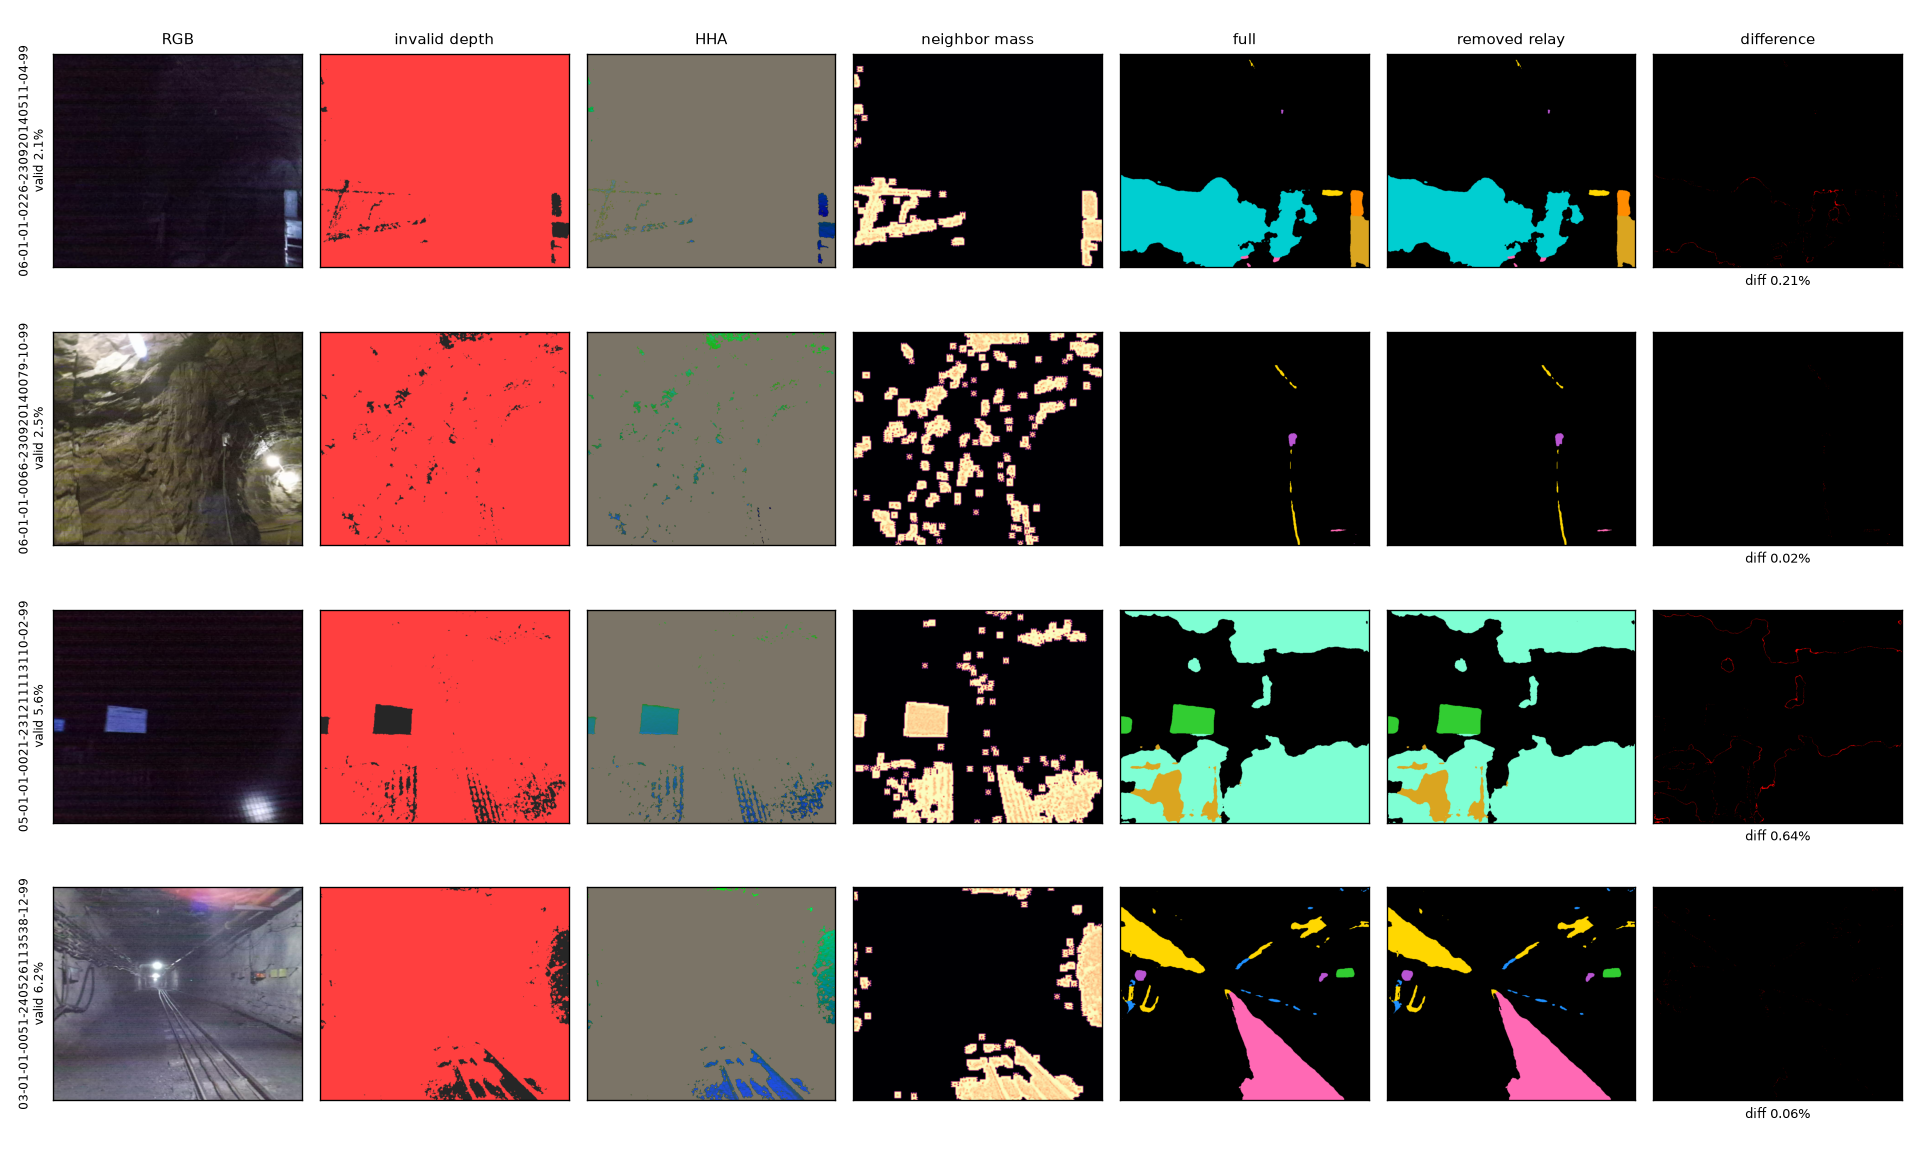
\includegraphics[width=\textwidth]{figures/contact.png}
\par\small 图 1  验证集低有效深度图像上的几何输入、Relay 权重和预测差异。
\end{center}
\begin{center}
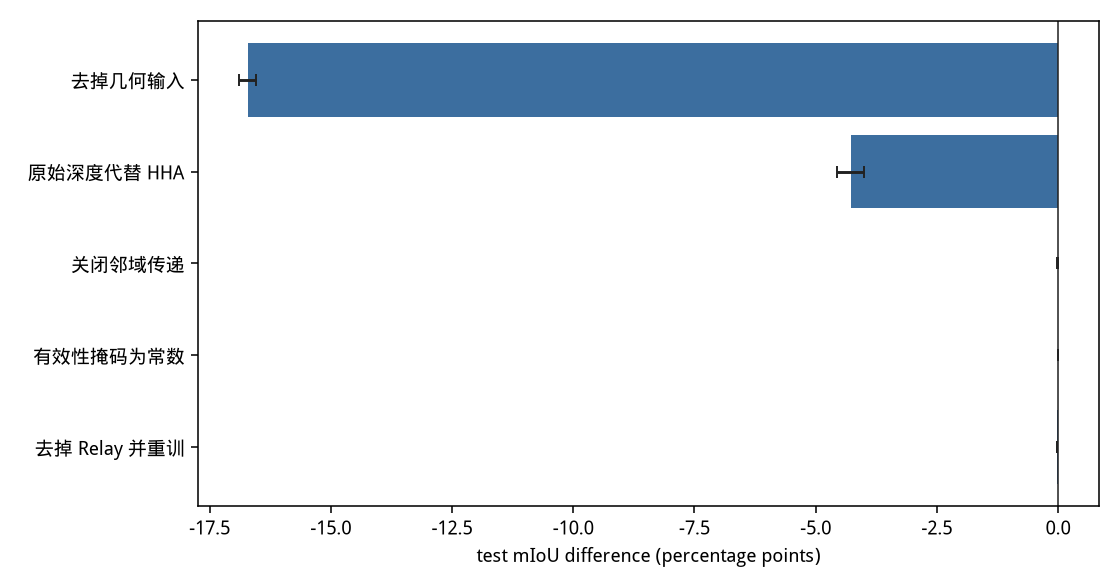
\includegraphics[width=\textwidth]{figures/delta-miou.png}
\par\small 图 2  测试集 16 类 mIoU 差，单位是百分点。误差线是三种子样本标准差。
\end{center}
\section*{8  结论}
去掉 Relay 并重训相对完整模型的 16 类 mIoU 差均值是 -0.02 个百分点，样本标准差是 0.01 个百分点。按事先写定的阈值，这是差异很小。

在这条标准下，Relay 的独立贡献很小。更简单的结构可以去掉这块模块。

机制变体的句子已在第 4 节按同一条规则写出。本文不把未达到稳定标准的单项差异解释成设计原因。

文件：结果 JSON 是 /root/autodl-tmp/MineSeg/v2/runs/relay\_retrain/results.json。分组阈值是同目录的 protocol.json。每个运行的验证历史、选择记录和 best.pth 在该目录的变体子文件夹里。论文的 Markdown、LaTeX、Word 和 PDF 在 /root/autodl-tmp/MineSeg/v2/paper\_relay\_retrain。

\end{document}
